
\item A particle A moves along a circle of radius \( R = 50 \) cm so that its radius vector \( \mathbf{r} \) relative to the point \( O \) (Fig. 1.5) rotates with the constant angular velocity \( \omega = 0.40 \) rad/s. Find the modulus of the velocity of the particle, and the modulus and direction of its total acceleration.
    \begin{center}
        % Since the image of the diagram is not provided, a placeholder is used here
        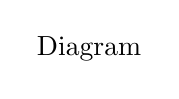
\begin{tikzpicture}
            \node at (0, 0) {Diagram}; % Replace this with the actual diagram or remove if not necessary
        \end{tikzpicture}
    \end{center}
    % If there are any subquestions, they would be added here. 
    % Given that there are no subquestions in the provided text, the enumerate environment is not used.
